\section{ScatterNets}\label{sec:ch2:scatternets}
% Let us define the pairs of authors here
  ScatterNets have been a very large influence on
  our work, as well as being quite distinct from the previous discussions on
  learned methods. They were first introduced by
  \citeauthor{bruna_classification_2011} in their work
  \cite{bruna_classification_2011}, and then were rigorously defined by Mallat
  in \cite{mallat_group_2012}. Perhaps the clearest explanation of them, and the most
  relevant to our work is in \cite{bruna_invariant_2013}.

  While CNNs have the ability to learn invariances to nuisance variabilities,
  their properties and optimal configurations are not well understood.
  It typically takes multiple trials
  by an expert to find the correct hyperparameters for these networks. A
  scattering transform instead builds well understood and well-defined invariances.

  We first review some of the desirable invariances before describing how a
  ScatterNet achieves them.

\subsection{Desirable Properties}
\subsubsection{Translation-Invariance}
  Translation is often said to be uninformative for classification --- an
  object appearing in the centre of the image \emph{should} be treated the same way as
  a similar object appearing near the corner of an image. This can be quantified
  by saying a representation $\Phi x$ is invariant to global translations $x_c(\bmu{u}) =
  x(\bmu{u}-\bmu{c})$ by $\bmu{c}=(c_1,c_2) \in \mathbb{R}^2$ if:
  % The first requirement for Scatternets - translation invariance
  \begin{equation}\label{eq:scat_trans_invariance}
    \norm{\Phi x_c - \Phi x} \leq C
  \end{equation}
  for some small constant $C>0$.
  Note that we may instead want only local translation-invariance and
  restrict the distance $|\bmu{c}|$ for which \eqref{eq:scat_trans_invariance}
  is true.

  Convolutional filters are naturally covariant to translations in the pixel space,
  so $\Phi x_c = (\Phi x)_c,\ \bmu{c} \in \mathbb{Z}^2$. Of course, natural objects
  exist in continuous space and are sampled, and any two images of the same
  scene taken with small camera disturbances are unlikely to be at integer pixel
  shifts of each other.

\subsubsection{Stability to Noise}
  Stability to additive noise is another useful invariance to incorporate,
  as it is a common feature in sampled signals. Stability is defined in terms of
  Lipschitz continuity, which is a strong form of uniform continuity for
  functions, which we briefly introduce here.

  Formally, a Lipschitz continuous function is limited in how fast it can change;
  there exists an upper bound on the gradient the function can take, although it
  doesn't necessarily need to be differentiable everywhere. The modulus operator
  $|x|$ is a good example of a function that has a bounded derivative and so is
  Lipschitz continuous, but isn't differentiable everywhere. Alternatively, the
  modulus squared has derivative everywhere but is not Lipshitz continuous as
  its gradient grows with $x$.

  \begin{figure}
    \begin{center}
      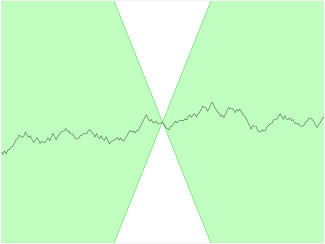
\includegraphics[scale=0.6]{\imgpath/Lipschitz_continuity.png}
      \mycaption{A Lipschitz continuous function}{There is a cone for this
              function (shown in white) such that the graph always remains entirely outside
              the cone as it is shifted across. The minimum gradient needed for this to hold
              is called the `best Lipschitz constant'.}
      \label{fig:lipschitz}
    \end{center}
  \end{figure}

  To be stable to additive noise, we require that for
  a new signal $x'(\bmu{u}) = x(\bmu{u}) + \epsilon(\bmu{u})$, there must exist
  a bounded $C>0$ s.t.
  % The second requirement - noise stability
  \begin{equation}\label{eq:ch2:scat_noise_stability}
    \|\Phi x' - \Phi x\| \leq C \|x' - x\|
  \end{equation}

\subsubsection{Stability to Deformations}
  Small deformations are important to be invariant to but this must be
  limited. It is important to keep intra-class variations small but not be so
  invariant that an object can morph into another (in the case of MNIST for
  example, we do not want to be so stable to deformations that 7s can map to
  1s).

  Formally, for a new signal
  $x_{\tau}(\bmu{u}) = x(\bmu{u}-\tau(\bmu{u}))$, where $\tau(\bmu{u})$ is a non
  constant displacement field (i.e.,\ not just a translation) that deforms the
  image, we require a $C_\tau>0$ s.t.
  % The third requirement - deformation stability
  \protect\begin{equation}\label{eq:scat_deformation_stability}
    \|\Phi x_{\tau} - \Phi x \| \leq C_\tau \|x\| \sup_{\bmu{u}} |\nabla\tau(\bmu{u})|
  \protect\end{equation}
  The term on the right $|\nabla\tau(\bmu{u})|$ measures the deformation
  amplitude, so the supremum of it is a limit on the global deformation amplitude.

\subsection{Definition}
  A Fourier modulus satisfies the first two of these requirements, in that it is
  both translation-invariant and stable to additive noise, but it is unstable to
  deformations due to the large support (infinite in theory) of the sinusoid basis functions it
  uses. It also loses too much information --- very different signals can all
  have the same Fourier modulus, e.g.\ a chirp, white noise and the Dirac delta
  function all have flat spectra.

  Another translation-invariant and stable operator is the averaging kernel
  which \Mallat\ use to make the zeroth scattering coefficient:
  \begin{equation}
    S[\emptyset]x \definedas x \conv \phitd_J\left(2^J \bmu{u}\right)
  \end{equation}
  which is translation-invariant to shifts less than $2^J$. It, unfortunately,
  results in a loss of information due to the removal of high-frequency content.
  This is easy to see as the wavelet operator from \eqref{eq:ch2:wave2} $\mathcal{W}x = \{ x \conv
  \phitd_J, x \conv \psitd_\lambda \}_\lambda$ contains all the information of
  $x$, whereas the zeroth scattering coefficient is simply the lowpass portion
  of $\mathcal{W}$.

This high-frequency content can be `recovered' by keeping the wavelet
coefficients. The wavelet terms, like a convolutional layer in a CNN, are only
covariant to shifts rather than invariant. This covariance happens in the real
and imaginary parts which both vary rapidly. Fortunately, its modulus is much
smoother and gives a good measure for the frequency-localized energy content at
a given spatial location\footnote{Interestingly, the modulus operator can often still be
inverted due to the redundancies of the complex wavelet transform \cite{waldspurger_phase_2012},
hence it does not lose any information.}. Unlike
the Fourier modulus, the complex wavelet modulus is stable to deformations due
to the grouping together of frequencies into dyadic packets
\cite{mallat_group_2012}.

We combine the wavelet transform and modulus operators into one operator
$\widetilde{\mathcal{W}}$:
\begin{align}
  \widetilde{\mathcal{W}}x &= \{ x \conv \phitd_J,\ |x \conv \psitd_\lambda| \}_\lambda \label{eq:ch2:wave3}\\
             &= \{ x \conv \phitd_J,\ U[\lambda]x \}_\lambda
\end{align}
where the $U$ terms are called the \emph{propagated} signals.
These $U$ terms are approximately invariant for shifts of up to $2^j$. \Mallat\ choose to
keep the same level of invariance as the zeroth-order coefficients ($2^J$)
by further averaging. This makes the first ordering scattering coefficients:
\begin{equation}
  S[\lambda_1]x \definedas U[\lambda_1]x \conv \phitd_J
  = |x \conv \psitd_{\lambda_1}| \conv \phitd_J
\end{equation}
Again this averaging comes at a cost of discarding high-frequency information,
this time about the wavelet sparsity signal $U[\lambda] = |x \conv
\psi_\lambda|$ instead of the input signal $x$. We can recover this information
by repeating the above process.
\begin{align}
  S[\lambda_1, \lambda_2]x &\definedas U[\lambda_2]U[\lambda_1]x \\
                           &=||x \conv \psitd_{\lambda_1}| \conv \psitd_{\lambda_2}| \conv \phitd_J
\end{align}
In general, let $p=(\lambda_1, \lambda_2, \ldots \lambda_m)$ be a path of length
$m$ describing the order of application of wavelets, and define:
\begin{align}
  U[p]x &= U[\lambda_m]U[\lambda_{m-1}]\cdots U[\lambda_1]x \\
        &= || \cdots |x \conv \psitd_{\lambda_1}| \conv \psitd_{\lambda_2} | \cdots
  \conv \psitd_{\lambda_m}| \label{eq:ch2:u_path}
\end{align}
and the $m$th order scattering coefficient along the path $p$ is $S[p]x = U[p]x
\conv \phitd_J$. Further, let $p+\lambda = (\lambda_1, \lambda_2, \ldots
\lambda_m, \lambda)$.  This allows us to recursively define the next set of
\emph{propagated} and \emph{scattering} coefficients by using $\widetilde{\mathcal{W}}$:
\begin{equation}
  \widetilde{\mathcal{W}}U[p]x = \{ S[p]x,\ U[p+\lambda]x \}_\lambda \label{eq:ch2:recursive}
\end{equation}
which is shown in \autoref{fig:ch2:scatternet_mallat}
  \begin{figure}
    \centering
      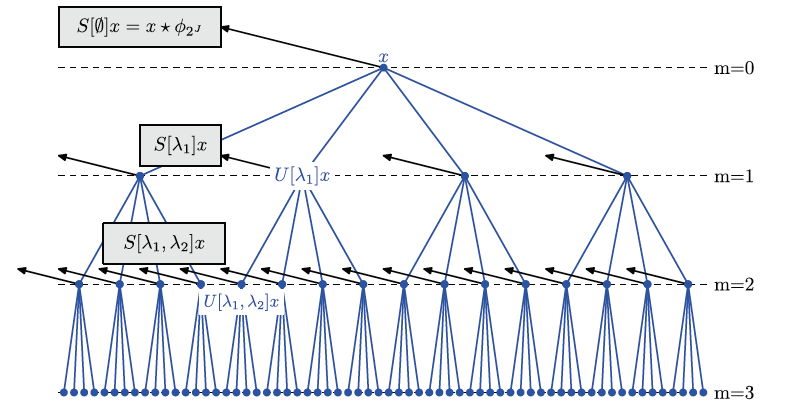
\includegraphics[width=\textwidth]{\imgpath/scatternet_diagram.png}
      \mycaption{The Scattering Transform}{Scattering outputs
               are the leftward pointing arrows $S[p]x$, and the intermediate
               coefficients $U[p]x$ are the centre nodes of the tree. Taken
               from \cite{bruna_invariant_2013}.}
      \label{fig:ch2:scatternet_mallat}
  \end{figure}

\subsection{Resulting Properties}
For ease, let us define the `$m$th order scattering coefficients' as $S_m$ which
is the set of all coefficients with path length $m$. Further, let $S$ be the set
of all scattering coefficients of any path length. The energy $\energy{Sx}$ we
then define as
\begin{equation}
  \energy{Sx} = \sum_p \energy{S[p]x}
\end{equation}
We can make $\mathcal{W}$ non-expansive with appropriate scaling. Define the energy $\energy{\mathcal{W}x}$ as
\begin{equation}
  \energy{\mathcal{W}x} = \energy{x\conv \phitd} + \sum_\lambda \energy{x \conv
  \psitd_\lambda}
\end{equation}
then by Plancherel's formula
\begin{equation}
  (1-\epsilon)\energy{x} \leq \energy{\mathcal{W}x} \leq \energy{x}
\end{equation}
For the Morlet wavelets originally used in \cite{bruna_invariant_2013},
$\epsilon=0.25$, for the $\DTCWT$ $\epsilon \approx 0$ (for the q-shift $\DTCWT$
it is 0, but for the biorthogonal $\DTCWT$ it is close to but not exactly 0).

\subsubsection{Translation-Invariance}
\newcommand{\shift}{\mathcal{L}_c}

This is proven in section 2.4 of \cite{mallat_group_2012}. We
have so far described the Scattering representation as being `translation-invariant
for shifts up to $2^J$'. We formalize this statement here.

For a 2-D averaging filter based on a father wavelet $\phitd$,
$\phitd_J = 2^{-J}\phitd\left(2^{-J}\xy\right)$ it is proven in Appendix B of
\cite{mallat_group_2012} that shifting
it by $\bmu{c}$, which we denote as $\mathcal{L}_c$, is Lipschitz continuous:
\begin{equation}
  \norm{\shift \phi_J - \phi_J} \leq 2^{-J+2}\lnorm{\nabla \phitd}{1}|\bmu{c}|
\end{equation}
where $\lnorm{\nabla \phitd}{1}$ is the $\ell_1$ norm of the grad of $\phitd$.

For simplicity, let us define $A_J x = \phitd_J \conv x$ and $Sx = A_J Ux$. Then we get:
\begin{align}
  \norm{S\shift x - Sx} & = \norm{\shift A_J Ux - A_J Ux} \\
                         &\leq \norm{\shift A_J - A_J}\norm{Ux} \\
                         & \leq 2^{-J+2}\lnorm{\nabla \phitd}{1}|\bmu{c}|\norm{x}
\end{align}
% as $\norm{Ux} \leq \norm{x}$.

\subsubsection{Stability to Noise}
As $\mathcal{W}$ is non-expansive and the complex modulus is also non-expansive
\begin{equation}
  \norm{\widetilde{\mathcal{W}}x - \widetilde{\mathcal{W}}y} \leq \norm{x-y} \label{eq:ch2:w_nonexpanse}
\end{equation}
We have already shown that $S$ is the repeated application of $\widetilde{\mathcal{W}}$ in
\eqref{eq:ch2:recursive}, we can then say
\begin{equation}
  \norm{Sx - Sy} \leq \norm{x-y}\label{eq:ch2:s_nonexpanse}
\end{equation}
making scattering non-expansive and stable to noise. With the $\DTCWT$, both
\eqref{eq:ch2:w_nonexpanse} and \eqref{eq:ch2:s_nonexpanse} are nearly
inequalities as $\epsilon$ is close to 0.

\subsubsection{Stability to deformations}
If $\mathcal{L}_\tau x = x(\xy -\tau(\xy))$ is an image deformed
by a diffeomorphism $\tau$ with $\norm{\tau}_\infty = \sup_u |\tau(\xy)|$
and $\norm{\nabla \tau}_\infty = \sup_u |\nabla \tau(\xy)| < 1$ then it is
proven in \cite{mallat_group_2012} that:
%
\begin{equation}
  \norm{ S \mathcal{L}_{\tau}x  - S x} \leq C P \norm{x} (2^{-J}\norm{\tau}_\infty + \norm{\nabla \tau}_\infty )
\end{equation}
%
where $P = \F{length}(p)$ is the scattering order and $C$ is a constant
(dependent on $J$). For deformations with small absolute displacement relative
to $2^J$, the first term disappears and we have:
\begin{equation}
  \norm{ S \mathcal{L}_{\tau}x  - S x} \leq C P \norm{x} \norm{\nabla \tau}_\infty  \label{eq:ch2:stability}
\end{equation}
This theorem shows that $S$ is locally Lipschitz stable to diffeomorphisms and in
the case of small deformations, it linearizes them.

\subsubsection{Energy Decay}
As $m \rightarrow \infty$ the invariant coefficients of path length $m$, $U_m$,
decay towards zero \cite{mallat_group_2012}:
\begin{equation}
  \lim_{m \rightarrow \infty} U_m = 0
\end{equation}
This is an important property that suggests that we can stop scattering beyond a
certain point. Experimental results \cite{bruna_invariant_2013} for
image sizes on the order of a few hundred pixels by a few
hundred pixels, $m=3$ captures about $99\%$ of the input energy. For many works
using scattering transforms after \cite{bruna_invariant_2013} such as
\cite{oyallon_deep_2015, oyallon_hybrid_2017, oyallon_scaling_2017}, setting
$m=2$ was found to be sufficient.

\subsubsection{Number of Coefficients}
While we have so far talked about non-sampled signals $x(\xy),\ \xy \in
\reals[2]$, in practice, we want to apply scattering to sampled signals $x[\nn],\
\nn \in \integers[2]$. The averaging by $\phitd_J$ means that we can subsample
$Sx$ by $2^J$ in each direction. However, now we need also need to index all the
paths $p$ that can be used to create the scattering coefficients. Limiting
ourselves to $m=2$ and using a wavelet transform with $J$ scales and $K$
discrete orientations the number of paths for each $S_m$ is the cardinality of
the set $p_m$:
\begin{align}
  n(p_0) &= 1 \\
  n(p_1) &= JK \\
  n(p_2) &= (J-1)K^2 + (J-2)K^2 + \ldots + K^2 \\
         &= \frac{1}{2}J(J-1)K^2
\end{align}
The reason $n(p_2) \neq J^2 K^2$ is due to the demodulating effect of the
complex modulus. As $|x \conv \psitd_\lambda|$ is more regular than $x \conv
\psitd_\lambda$, $|x \conv \psitd_\lambda| \conv \psitd_{\lambda'}$ is only
non-negligible if $\psitd_{\lambda'}$ is located at lower frequencies than
$\psitd_\lambda$. This means we can discard over half of the scattering paths as
their value will be near zero.

Summing up the above three equations and factoring in the reduced sample rate
allowable due to averaging, for an input with $N$ pixels, a second-order scattering
representation will have $N2^{-2J}\left(1+JK+\frac{1}{2}J(J-1)K^2 \right)$
pixels. \autoref{tab:ch2:scat_redundancy} shows some example values of the
ScatterNet redundancy for different $J,K$ and scattering order $m$.

\begin{table}
  \centering
  \mycaption{Redundancy of Scattering Transform}{Shows the number of output
  channels $C_{out}$ and number of pixels per channel $N_{out}$ for different
  scattering orders $m$, scales $J$, and orientations $K$ for a single channel
  input image with $N$ pixels.}
  \label{tab:ch2:scat_redundancy}
\begin{tabular}{l l l l l l l}
  \toprule
  m & J & K & \hphantom{abc} & $C_{out}$ & $N_{out}$ \\
  \midrule
  1 & 2 & 6 && 13 & $N/16$ \\
  1 & 2 & 8 && 17 & $N/16$\\
  2 & 2 & 6 && 49 & $N/16$\\
  2 & 2 & 8 && 81 & $N/16$ \\
  2 & 3 & 6 && 127 & $N/64$\\
  2 & 3 & 8 && 217 & $N/64$\\
  3 & 3 & 6 && 343 & $N/64$\\
  3 & 3 & 8 && 729 & $N/64$\\
  \bottomrule
\end{tabular}
\end{table}
